\section{Lissage d'une image}

\begin{enumerate}[questions, start=11]
\item On implémente le lissage par convolution sous Scilab dans le fichier \verb|functions.sci|:
  \begin{itemize}
  \item la fonction \verb|convolKernel(sigma, eta)| renvoie une matrice carrée $G$ dont les coefficients sont de la forme 
  \[ \dfrac{1}{2\pi\sigma^2}\exp{\left( -\dfrac{k^2 + l^2}{2\sigma^2} \right)} \]
  et vérifient tous $G_{i,j} \geq \eta$ ou sont nuls (où $\sigma =$ \verb|sigma| et $\eta = $ \verb|eta|);
  \item la fonction \verb|reflectMat(I, n)| renvoie une matrice au centre de laquelle on retrouve $I$. Les lignes et colonnes restantes sont remplies à partir de celles de $I$, par \og{}symétrie d'axe les bords de $I$\fg{};
  \item la fonction \verb|blur(I, sigma, eta)| calcule la convolée de $I$ par la gaussienne de paramètre $\sigma = $ \verb|sigma| tronquée à la précision $\eta = $ \verb|eta|.
  \end{itemize}
On peut voir quelques exemples sur des images ci-dessous:
\begin{figure}[!h]
\centering
  \begin{subfigure}{0.3\textwidth}
  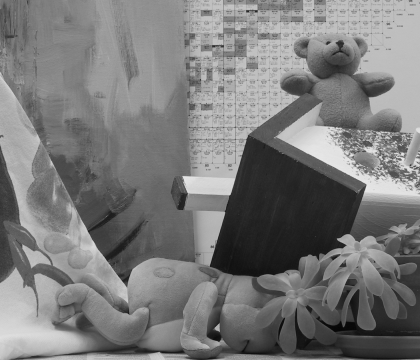
\includegraphics[width=\textwidth]{img/teddy-noblur.png}
  \caption{Image originale}
  \end{subfigure}\hfill
  \begin{subfigure}{0.3\textwidth}
  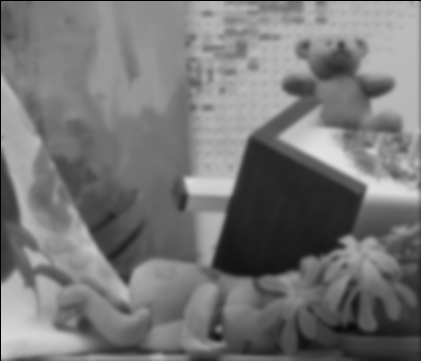
\includegraphics[width=\textwidth]{img/teddy-blur-2.png}
  \caption{Flou avec $\sigma = 2$}
  \end{subfigure}\hfill
  \begin{subfigure}{0.3\textwidth}
  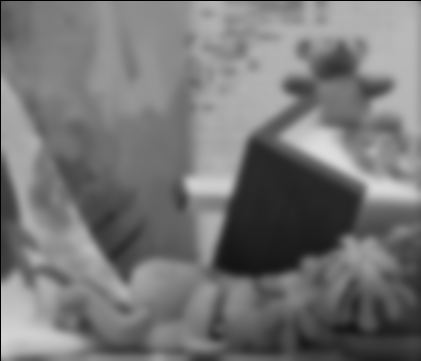
\includegraphics[width=\textwidth]{img/teddy-blur-4.png}
  \caption{Flou avec $\sigma = 4$}
  \end{subfigure}\\
  
  \begin{subfigure}{0.3\textwidth}
  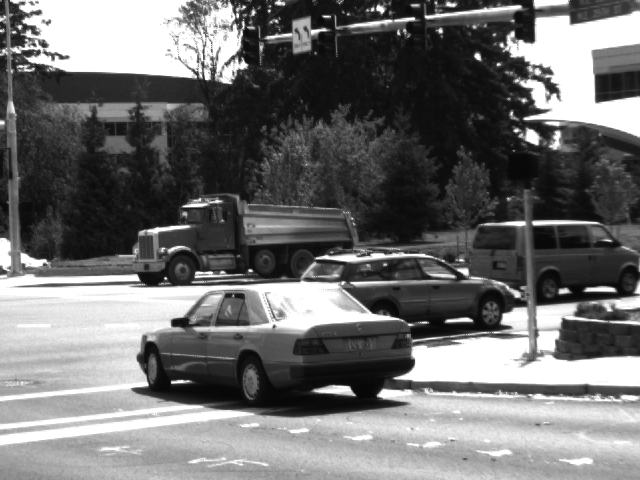
\includegraphics[width=\textwidth]{img/dumptruck-noblur.png}
  \caption{Image originale}
  \end{subfigure}\hfill
  \begin{subfigure}{0.3\textwidth}
  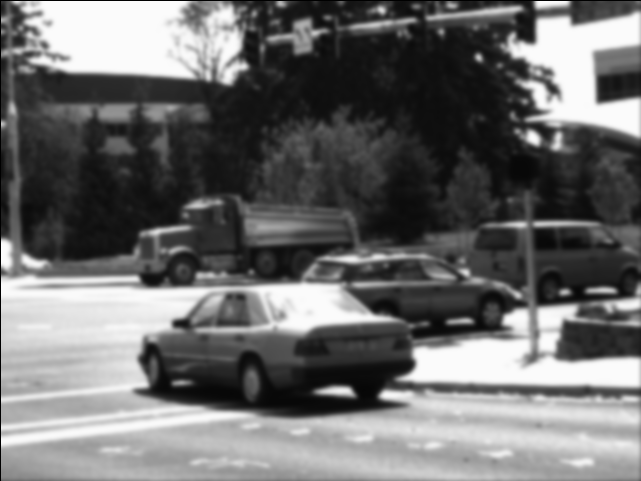
\includegraphics[width=\textwidth]{img/dumptruck-blur-2.png}
  \caption{Flou avec $\sigma = 2$}
  \end{subfigure}\hfill
  \begin{subfigure}{0.3\textwidth}
  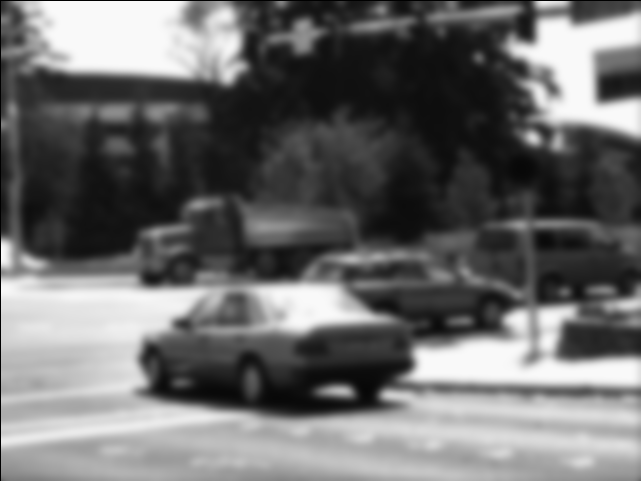
\includegraphics[width=\textwidth]{img/dumptruck-blur-4.png}
  \caption{Flou avec $\sigma = 4$}
  \end{subfigure}\\
  
  \begin{subfigure}{0.3\textwidth}
  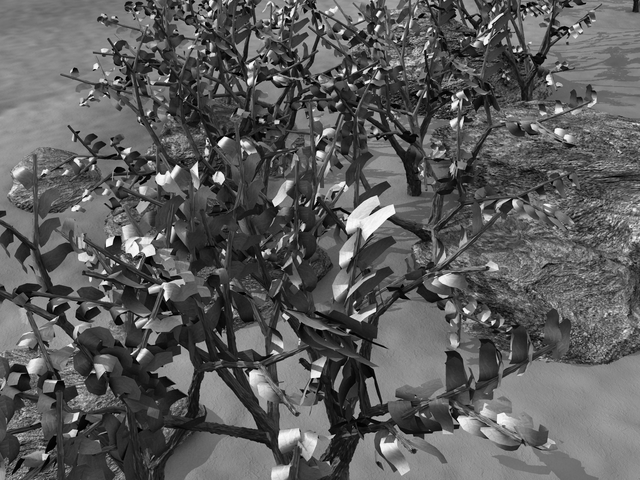
\includegraphics[width=\textwidth]{img/grove-noblur.png}
  \caption{Image originale}
  \end{subfigure}\hfill
  \begin{subfigure}{0.3\textwidth}
  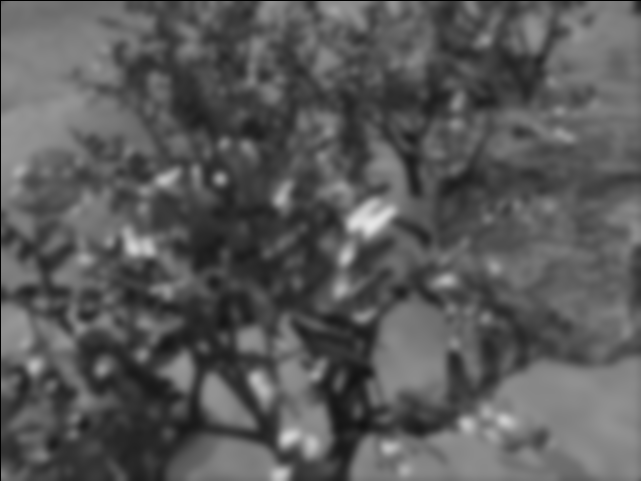
\includegraphics[width=\textwidth]{img/grove-blur-4.png}
  \caption{Flou avec $\sigma = 4$}
  \end{subfigure}\hfill
  \begin{subfigure}{0.3\textwidth}
  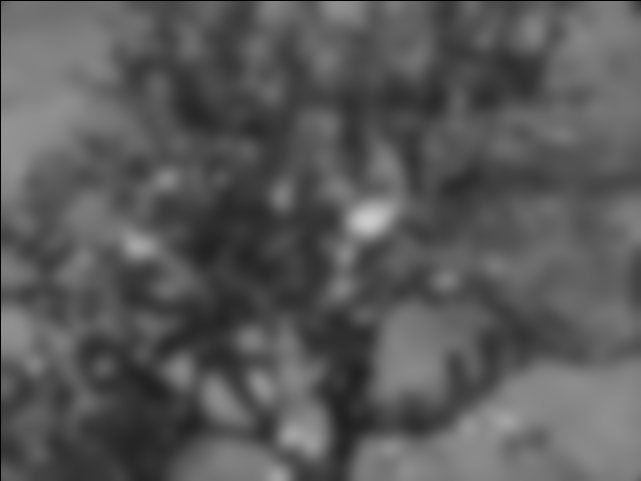
\includegraphics[width=\textwidth]{img/grove-blur-8.png}
  \caption{Flou avec $\sigma = 8$}
  \end{subfigure}
\caption{Quelques illustrations du lissage gaussien.}
\end{figure}
\end{enumerate}

\begin{enumerate}[questions, start=13]
\item Il faut mettre les deux couples d'images. Trop tard ce soir... :p
\end{enumerate}